% simple document template
\documentclass[12pt]{article}
\usepackage{tikz}
\usetikzlibrary{graphs}
\usetikzlibrary {mindmap}
\usepackage{hyperref}
\begin{document}

\title{Flips Websites}
\author{Pengfei}
\date{\today}
\maketitle

\tableofcontents

% /usr/local/texlive/2023/bin/universal-darwin/pdftex
% /usr/local/texlive/2023/texmf-var/web2c/pdftex
% /usr/local/texlive/2023/texmf-var/fonts/map/pdftex
% /usr/local/texlive/2023/bin/universal-darwin/pdftex
% /usr/local/texlive/2023/texmf-dist/tex/generic/pdftex
% ==========[Section Potential]===========
\section{Potential}
\subsection{ROI}
\paragraph{How many websites}~\\
\begin{verbatim}
    1. 1B websites
    2. 2B houses
    3. 7B videos on tictoc
\end{verbatim}

\subsection{Goal}
\begin{itemize}
    \item 1. 2024: make \$1000 to by a mac book air M3 chips
\end{itemize}

\subsection{How to make it work}
\begin{itemize}
    \item 1. Keyword choice and SEO
    \item 2. Focus on keywords solve real problems
    \item 3. Find a keyword:
    \item 4. low competition good search vol and solve real problems
    \item 5. Make more sites to blank page 1 of google
    \item 6. Bad things happen: depend on google algorithm
    \item 7. Make a website
\end{itemize}

\subsection{Flip markets}

Takes ~15\% fee
\begin{itemize}
    \item 1. Lead Spring
    \item 2. \href{https://flippa.com/}{Flippa}
    \item 3. Flip content
    \item 4. Flip videos
\end{itemize}

\subsection{Google}
\paragraph{Google search trends}~\\

\begin{figure}
    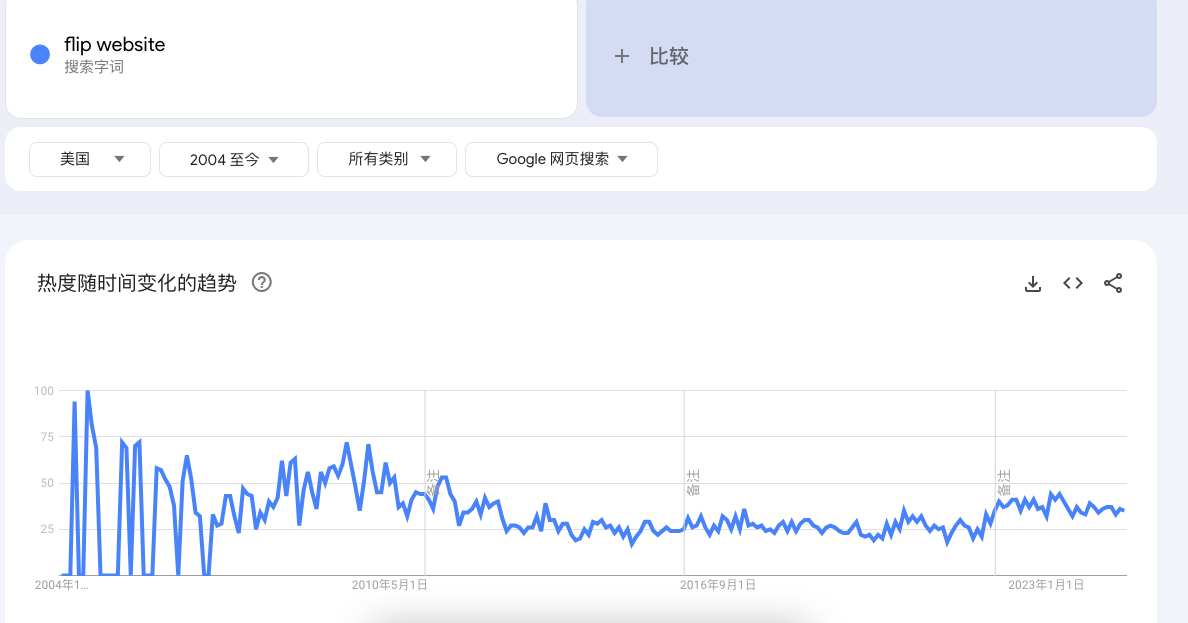
\includegraphics[width=0.5\textwidth]{./images/trend_flip_websites.png}
    \caption{Google search trends}
\end{figure}

Key findings:
\begin{itemize}
    \item 1. gradually increases
    \item 2. every 6 years major update to google
\end{itemize}

\subsection{Example}
\paragraph{Ideas}~\\

Guidance: some topic I am interested or some digital product I can improve

\begin{itemize}

    \item \href{https://www.mybabyboutique.us/}{MyBaby.com}
    \item \href{https://www.printable-ruler.net/}{Printable Ruler(I can customize the rulers!)}
\end{itemize}

\subsection{Buy a website vs build a website}
\begin{itemize}
    \item 1. Buy a website: doman / google rank / web SEO structure / stable traffic
    \item 2. Build a website: cheaper
\end{itemize}

% ==========[Section SEO]===========
\section{SEO}

\begin{itemize}
    \item 1. Great content
    \item 2. Use keywords on your page
    \item 3. Page load time
    \item 4. SEO is about keywords: find 5 keywords 
    \item 5. find keyword using google auto complete


\end{itemize}
% ==========[Section Google ranking]===========
\subsection{Google ranking}

Google has published its ranking criterias.
\begin{itemize}
    \item 1. Domain name
    \item 2. Google rank
    \item 3. Web SEO structure
    \item 4. Stable traffic
    \item 5. Content
\end{itemize}

\subsection{Keywords}
\begin{itemize}
    \item 1. Keyword volumn: how many people search for this keyword
    \item 2. Keyword competition: how many people are competing for this keyword
    \item 3. traffic potential: how much traffic can I get from this keyword if rank \#1
\end{itemize}

% ==========[Section Web Hosting]===========
\section{Web Hosting}

\subsection{Concepts}

I should choose VPS for beginer.
\begin{itemize}
    \item 1. VPN: virtual private Network
    \item 2. CDN: content delivery network
    \item 3. VPS: virtual private server(share of machines)
    \item 4. VPC: virtual private cloud(actual machine / cloud)
\end{itemize}

\paragraph{Tools}~\\
\begin{itemize}
    \item 1. \href{https://www.vpsbenchmarks.com/compare/ec2_vs_vultr}{Compare VPS}
\end{itemize}


\subsection{VPS Providers}
\begin{itemize}
    \item 1. IONOS.com / bluehost
    \item 2. AWS EC2: costly, should for medium projects
    \item 3. linode: too old
    \item 4. digital ocean: a little old
    \item 5. \tikz \node[fill=green!10!white]{vultr: good};
\end{itemize}

\subsection{Costs}
\begin{itemize}
    \item 1. IONOS.com / bluehost
    \item 2. SSL
    \item 3. Domain name
    \item 4. Email address
    \item 5. Backups: for security
    \item 6. Domain privacy: hides email/phone number
\end{itemize}

\subsection{Solution}
\begin{itemize}
    \item 1. IONOS.com
    \item 2. Bluehost
    \item 3. WordPress + REST API + FLASK
\end{itemize}

\subsection{Scrum}
\href{https://create.microsoft.com/en-us/learn/articles/four-tips-to-track-projects-in-excel}{mange scrum project using excel}

% ==========[Section References]===========
\section{References}
\subsection{Web}
\begin{itemize}
    \item 1. \href{https://www.youtube.com/watch?v=UaJIkkZbaEY}{Matt Diggity}
    \item 2. \href{https://jaserodley.com/website-flipping/}{Jase Rodley}
    \item 3. \href{https://www.godaddy.com/}{Go Daddy: search for unused domain}
\end{itemize}
    
\end{document}